\section{Data Process Results}
\label{sec:data process}

In the previous sections, we have introduced different algorithms for band adaptation. 
In this section, we introduce the metrics for evaluation and compare the proposed schemes with the data collected in
\ref{sec:experiment design}.

Throughput is the most important metric for any kind of networks and very sensitive to customers. In multi-band scenario, the object is to find the band has the best throughput.  
\emph{Accuracy} is defined as the percentages of predict best band match the measured best band.

The throughput will be normalized across the bands to remove the divergence of the radios. Then the data will be divided into different subsets for the algorithms introduced in 
\ref{sec:model}.

%Ideal channel based process and accuracy computation
For \emph{Ideal Channel based Algorithm}, it does not need a whole information, including the throughput. It fits for every data point.
This algorithm is used in every data points and the \emph{Accuracy} is counted through all the prediction and measured data. The algorithm is independent to the environment, it could be used anywhere.
%ML and LB algorithms process and accuracy computation
For \emph{Machine Learning Algorithm} and \emph{Location Based Algorithm}, a fixed amount of the in-field data is used as test set and part of remaining data is used for training set. The \emph{Accuracy} performance is counted as the correct prediction of the test set. 
The performance of these algorithms is dependent on the amount of training set. In figure \ref{fixme} we show the variation of \emph{accuracy} of different amount of training set.



\begin{figure}
\centering
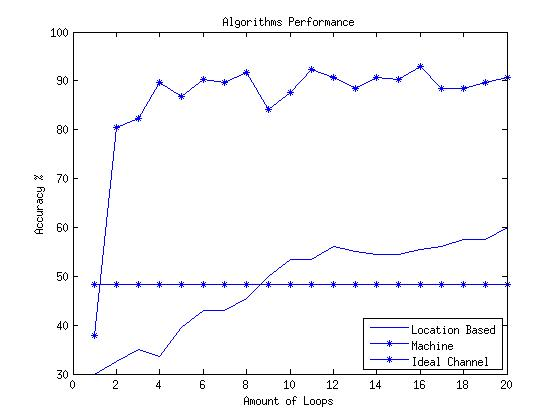
\includegraphics[width=85mm]{figure/performance_al}
\caption{Performance of Algorithms}
\label{fig:performance}
\end{figure}


The x-axis in \ref{fig:performance} is the number of loops the mobile node traveled through the park. We could see as the loops increase, the accuracy of the two algorithms go up. 
\emph{Machine Learning Algorithm} has better accuracy than \emph{Location based Look up Algorithm} in the same training data. The cost of \emph{Machine Learning Algorithm} is the training resource and time for training.

The data set is also divided into multiple regions to test the \emph{Split Region Machine Learning Algorithm}. There are 8 regions shown in \ref{fixme}
in different colors.




%signal level in the measured signal level interregional. We evaluate both the theoretic results from path loss equation and the context-aware base framework in this scenario.

%\emph{Performance Improvement} is the percents of throughput of multi-band over single band.


%\subsubsection{Indoor Experiments} 
%We first use the signal level of test data in different band to calculate the signal level of different bands. Then we use the signal level database to predict the signal level. The results from the two methods are compared with the measured signal. The graph shows the calculation results, the context-aware results for fixme set of training data, and the measured results.
%
%%fixme graph of calculation, context-aware and measured
%
%The amount of information in context-aware database will influence the accuracy of results. How much information is enough for the prediction for the signal is an interesting question. We put the same test data into different size context-aware database to produce the output signal level in different bands. The graph shows the signal level prediction in different context-aware database and the measured results.
%
%%fixme graph of context-aware signal in different loops, different loops in different curves
%
%Following graph shows the \emph{Accuracy in Signal Level} for different size context-aware database in indoor experiments.
%
%% fixme hint graph of accuracy in signal level
%
%
%Through the multi-band framework, we analyze the influence of time window for the performance estimation. We show the estimation in different size of time window and the measured throughput.
%
%%fixme estimation of different time window and measured throughput
%
%
%If we implement the band switching, the improvement is shown in the following graph,
%
%%fixme multi-band improvement
%
%
%
%
%
%
%
%
%
%
%
%
%
%%fixme could we show some results only rely on emulator data??? such as the signal level prediction? show in the ideal channel state, the pathloss equation calculation make more sense???????????????????????????????????
%
%
%
%
%
%
%\subsubsection{In-field Experiments} 
%In the previous section, we analyze and shows the results of indoor experiments. In this section, we will introduce the results of in-field experiments.
%We also has the same metric as in-door experiments for evaluation. 
%The graph shows the calculation results, the context-aware results for fixme set of training data, and the measured results.
%
%%fixme graph of calculation, context-aware and measured
%
%In in-field status, there are more factors will influence the signal level. We analyze the influence of information amount for context-aware database in in-field situation and shows in the following graph.
%
%%fixme graph of context-aware signal in different loops, time/number as x-axis
%
%Following graph shows the \emph{Accuracy in Signal Level} for different size context-aware database in in-field experiments.
%
%% fixme hint graph of accuracy in signal level
%
%
%Through the multi-band framework, we analyze the influence of time window for the performance estimation. We show the estimation in different size of time window and the measured throughput.
%
%%fixme estimation of different time window and measured throughput
%
%
%
%The potential improvement is shown in the following graph,
%
%fixme improvement for multiband switich



%Detail may not useful
%Parsing script
%In our experiments, we are constantly collecting large amounts of data, including the received signal level, current location, velocity, and time of day. Working with the memory-limited Gateworks boards, it became necessary to implement a solution to collect large amounts of data without exhausting the available memory space on the boards. Thus, we compiled a script to parse an undetermined number of data files containing the raw data collected from the ongoing experiments. Utilizing the Perl programming language, which the Gateworks boards are capable of running, the script scans every file in a directory we specify and parses them, looking specifically for signal level, lat/long location, velocity, and time data recorded from the experiments. Upon finding this information, the script reformats the data by placing it into a .csv file. Additionally, using the location data, the script calculates the  distance between the transmitting and receiving boards and adds this information to the .csv file. Upon parsing the data, the raw experimental data files can simply be delete from memory, freeing up space for the data of subsequent experiments.

%Activity monitor script
%For in-situ experiments, the need became apparent to track the number of new incoming packets and compare it with the number of previously received packets. Additionally, this needed to be done for each of the four wireless radios on the board. In doing this, we identify the most efficient frequency band to transmit data. To implement this system, a script was needed to run efficiently in the background while experiments were taking place. To achieve this, we wrote a bash shell script to run directly on the board without relying on any higher level programming language that could potentially cause greater performance overhead. As a result, the script only consumes one to two percent of CPU resource. The script begins by examining the received bytes across each radio for a length of 30 seconds and placing the bytes received each second on a new line in a file. Upon the completion of the 30 second buffering time period, the next second of received bytes on each radio is read and compared with the last 30 seconds of received data. This ratio of the most recent received data to old received data is then calculated and written to four files, one for each radio, for its subsequent use in selecting which radio to transmit/receive from.

